\section{Resampling Study}

To test the ecological validity of findings in experiment 1 and 2 we designed a resampling study 
based on European Values Survey (EVS) data.

EVS is a large scale, cross-national survey on human values administered in almost 50 countries
across Europe.
It covers a wide range of human values and topics such as family, work, environment, perceptions of life, 
politics and society, religion and morality, national identity.
It is a high quality survey widely used for comparative studies between European countries.
Furthermore, it is accessible free of charge and it represents the type of data social scientist 
regularly work with.

Variables in the EVS data are not generated artificially from continuous normal distributions, 
or predefined Factor Analysis models, but are discrete numerical and categorical items following a 
variety of distributions.
By using data gathered for an actual survey, we could study whether the relative performances of 
the imputation methods, displayed in the simulation studies, changed when deployed for real data 
research.

It is useful to think of a research scenario to go along the resampling study.
Imagine a researcher that wants to test some hypothesis derived from sociological theory and 
decides to analyse a large comparative social survey to address their research question.
The data has missing values and decisions must be made on how to treat them.
The researcher wants to use an imputation procedure that discards as little information as possible 
from the observed data, while making as little arbitrary decisions as possible regarding which 
predictors to include in the imputation models.
This researcher will inevitably have to decide which imputation method to use and how to specify it.

\subsection{Resampling Study Procedure} \label{resProc}

The resampling study followed a similar strategy to that used in for the simulations. 
To assess the statistical validity of the different imputation methods we repeated the 
following steps 1000 times ($R = 1000$):

\begin{enumerate}
	\item Data generation: A bootstrap sample $\bm{Z}^{*}$ is generated by sampling with replacement $n$ 
		observations from a pre-processed EVS data-matrix. 
		Part of the pre-processing step is the imputation of the extant missing data to obtain a pseudo-fully 
		observed input data matrix so that $\bm{Z}^{*}$ has no missing values;
	\item Missing data imposition: Missing values are imposed on a given number of target variables
		in $\bm{Z}^{*}$, according to some response model (see below), and $\bm{Z}^{*}_{miss}$ is 
		obtained;
	\item Imputations: Each method described in section 2 is used to deal with missing values
		in $\bm{Z}^{*}_{miss}$.
	\item Analysis: Two analysis models are fitted to the differently imputed data.
		Their parameter estimates are pooled across the differently imputed datasets, for the MI methods, 
		and stored along with the estimates obtained after using single imputation methods, complete case 
		analysis, and the Gold Standard method.
\end{enumerate}

	The average estimates, over the $R$ repetitions, obtained with the Gold Standard approach were considered 
	as ``true" reference values of the parameters in the analysis models.
	The $R$ estimates obtained with all other methods were used to compute the performance measures described 
	in section \ref{criteria}.

\subsubsection{Data preparation and generation}
	For this study we used the third pre-release of the 2017 wave of EVS data \citep{EVS:2017}.
	The original dataset contained 55,000 observations in 34 countries.
	We selected only the four founding countries of the European Union included in the dataset (France, Germany,
	Italy, and the Netherlands) and excluded all columns of the data that were either duplicated
	information (recoded versions of other variables), or meta data (e.g. time of interview,
	mode of data collection). 

	All originally missing values were filled in with a run of a single imputation predictive mean matching (PMM) 
	algorithm to obtain a pseudo fully-observed dataset.
	PMM was chosen for the task as it is a flexible imputation method that maintains the distributional 
	characteristics of the original data.
	Bias and uncertainty introduced by this procedure is not relevant for the present study as the data matrix
	obtained after the single PMM run is treated as the population data.
	
	At the end of this data cleaning process, we obtained a fully-observed dataset
	of 8045 observations ($n$), across 4 countries, and 243 variables ($p$).
	
	For every repetition of the first step in the resampling procedure, a bootstrap sample $\bm{Z}^{*}$ was 
	generated by sampling with replacement $n$ observations from the EVS population data.

	\paragraph{Conditions}
	There were only two conditions for the resampling study: low and high dimensional data imputation.
	As the number of predictors in the data is fixed ($p = 243$), the dimensionality of the data was 
	changed by defining different sizes for the sample taken from the pseudo-fully observed data in
	step 1.
	We chose two values for $n$, namely $1000$ and $300$, corresponding to the low and high 
	dimensional condition.

\subsubsection{Analysis models}

	To define plausible analysis models we searched for analysis models that have been used in published articles
	testing sociological theories on the EVS data.
	The search was performed by screening the repository of publications using EVS data available on the EVS website.

	As a results, we defined two linear regression models, model 1 and 2, of the same form:
	
	\begin{equation}
		y = \beta_{0} + \beta_{1} x_{1} + \bm{\beta}_{-1} \bm{X}_{-1}  \label{eqn:lm}
	\end{equation}
	
	where a dependent variable $y$ is regressed on a variable of interest $x_{1}$ and a set of control variables
	$\bm{X}_{-1}$.
	In this scenario, $\beta_{1}$ is a focal parameter that a researcher wants to use to test some hypothesis.

	The first version of linear model \ref{eqn:lm}, model 1, was inspired by \cite{koneke:2014}:
	$y^{(1)}$, its dependent variable, was a 10-point EVS item measuring euthanasia acceptance 
	(`Can this always be justified, never be justified, or something in between?');
	the predictor of interest $x^{(1)}_{1}$ was a 4-point item measuring the self-reported importance of religion in 
	one's life;
	the matrix of covariates $\bm{X}^{(1)}_{-1}$ contained a selection of control variables
	(trust in the health care system, trust in the state, trust in the press,
	country, sex, age, education, and religious denomination).

	This model represents a plausible analysis a researcher would perform to test an hypothesis regarding the 
	effect of religiosity on the acceptance of end-of-life treatments.

	Model 2, the second version of the linear model in equation \ref{eqn:lm}, was inspired by \cite{immerzeel:2015}.
	The dependent variable $y^{(2)}$ was an harmonized variable constructed by EVS to describe the respondents' 
	tendency to vote left or right wing parties, expressed on a 10-point left-to-right continuum.
	The predictor of interest $x^{(2)}_{1}$ was a composite mean scale measuring respondents attitudes toward immigrants 
	and immigration (`nativist attitudes scale').
	The scale was obtained by taking the average of respondents expressed agreement, on a scale from 
	1 to 10, to three items: `immigrants take jobs away from natives', `immigrants increase crime problems', and 
	`immigrants are a strain on welfare system'.
	The control variables used were: 
	attitudes toward low and order, attitudes toward authoritarianism, interest in politics, level of political activity,  
	country, sex, age, education, employment status, socio-economic status, importance of religion in life, 
	religious denomination, and the size of town where interview was conducted.

	A researcher might fit this model and look at the value and standard error of $\beta^{(2)}_{1}$, 
	the `nativist attitude' regression coefficient, to test an hypothesis regarding the effect of xenophobia on voting 
	tendencies.

\subsubsection{Missing data imposition}

	Missing data were imposed on 6 variables according to the same strategy described in \ref{sub_missing}.
	The variables target of missing value imposition were the euthanasia acceptance item $y^{(1)}$ and the 
	left-to-right voting tendency $y^{(2)}$, the two dependent variables in model 1 and 2; 
	religiosity ($x^{(1)}_{1}$, focal and control variable in model 1 and 2 respectively), 
	and the three items making up the ``nativist attitudes'' scale (focal predictor $x^{(2)}_{1}$
	in the second model).

	The response model form was the same as in equation \ref{eqn:rm} and three variables were included in $\tilde{X}$: 
	age, education, and an item measuring trust in new people. 
	These aspects may plausibly influence response tendencies in participants: 
	older people usually have higher item non-response rates than younger people;
	lower educated people tend to have higher item non-response rates than higher educated people;
	people with less trust in strangers are assumed to have higher item non-response tendency as they
	are likely to withhold more information from the interviewer (a stranger).

\subsubsection{Imputation}
	
	Missing values were dealt with according to all the methods described in section 2.
	Here, we describe some key details in the algorithms specifications.

	\paragraph{Convergence}

	As for the simulation studies, convergence of the imputations was assessed in a pre-processing step.
	Before running the actual resampling study, 10 datasets were sampled from the EVS populaton data and missing 
	values were imposed.
	Missing values were then imputed by running 5 parallel imputation chains for each Multiple Imputation 
	method.
	Convergence was checked by plotting the mean of the imputed values for each variable in each stream, against the 
	iteration number.
	This procedure was performed only for condition 2, the high-dimensional one, under the assumption that convergence
	would be faster in the low-dimensional set up.

	After the convergence check, we decided to run the algorithms for the regular experiment run for 60 iterations 
	before saving the multiply imputed datasets, although most methods achieved convergence well before that number 
	of iterations.

	\paragraph{Tuning penalty parameters}

	The ridge penalties used in the bridge algorithm were chosen with the same cross-validation procedure 
	described for experiment 1 and 2.
		
	IURR and DURR used a lasso formulation of the frequentist regularized regression and
	a 10-fold cross-validation procedure was performed at every iteration to choose the penalty parameter.

	\paragraph{Blasso hyper-parameters}

	In order to maintain consistency with previous research, the hyper-parameters in \ref{eqn:sigprior},
	\ref{eqn:tauprior}, and \ref{eqn:rhoprior} were specified as in \cite{zhaoLong:2016}: $(a,b)=(0.1, 0.1)$, 
	$(r,s)=(0.01, 0.01)$, and $(g,h)=(1,1)$.

	\paragraph{MI-PCA Number of components}

	In the MI-PCA algorithm, enough components were extracted to explain 50\% of the total variance in the data.

	\paragraph{missForest iterations and number of trees}

	As in the simulation studies, the maximum number of iterations was set to 20 and the number of trees
	for the random forest was set to 100.

\subsection{Results}

	\subsubsection{Single Parameter of interest}

	Figures \ref{fig:exp4bias} and \ref{fig:exp4ci} report the PRB and the CIC for parameters $\beta^{(1)}_{1}$ and 
	$\beta^{(2)}_{1}$, the focal regression coefficients in the two models.

	Most of the MI methods resulted in negligible biases ($|PRB| < 10\%$) for both parameters in all conditions.
	The only two exceptions were bridge and MI-RF: 
	the former was very competitive in condition 1, the low dimensional one, but led to extreme bias and 
	over-coverage in the high dimensional condition for $\beta^{(2)}_{1}$; 
	the latter provided the largest PRBs and worst CIs (under) coverage for the focal regression coefficients among 
	the other MI methods, and it was consistently outperformed even by Complete Case analysis.
	missForest also displayed contained focal parameter biases.

	DURR and IURR gave inconsequential biases for both parameters in all conditions, with PRBs that were
	often at least half in size as the ones obtained with the other methods, outperforming even MI-OP in the high 
	dimensional condition for $\beta^{(2)}_{1}$.

	For $\beta^{(2)}_{1}$ in model 2, both IURR and DURR remained fairly competitive in terms of coverage 
	with CICs close to nominal levels, but the advantage they showed in terms of bias was not carried over to 
	this criterion.
	Both MI-PCA and Blasso provided CICs either equal or closer to nominal than the ones obtained with
	IURR and DURR in almost all conditions.

	As for $\beta^{(1)}_{1}$, all MI methods showed signs of under-coverage with CIC smaller than the threshold 
	value 0.94.
	Although coverage of the true values was not great for any of the methods selected, the Gold Standard
	confidence intervals were also under-covering the true value of $\beta^{(1)}_{1}$.
	This was likely due to the right-skewed nature of the distribution of the dependent variable (euthanasia 
	acceptance).
	Most MI imputation methods achieved coverages similar to that of the Gold Standard method, and more importantly 
	their relative difference, compared to the GS coverages, was in line with what can be seen for $\beta^{(2)}_{1}$.

\begin{figure}[h]
	\centering
	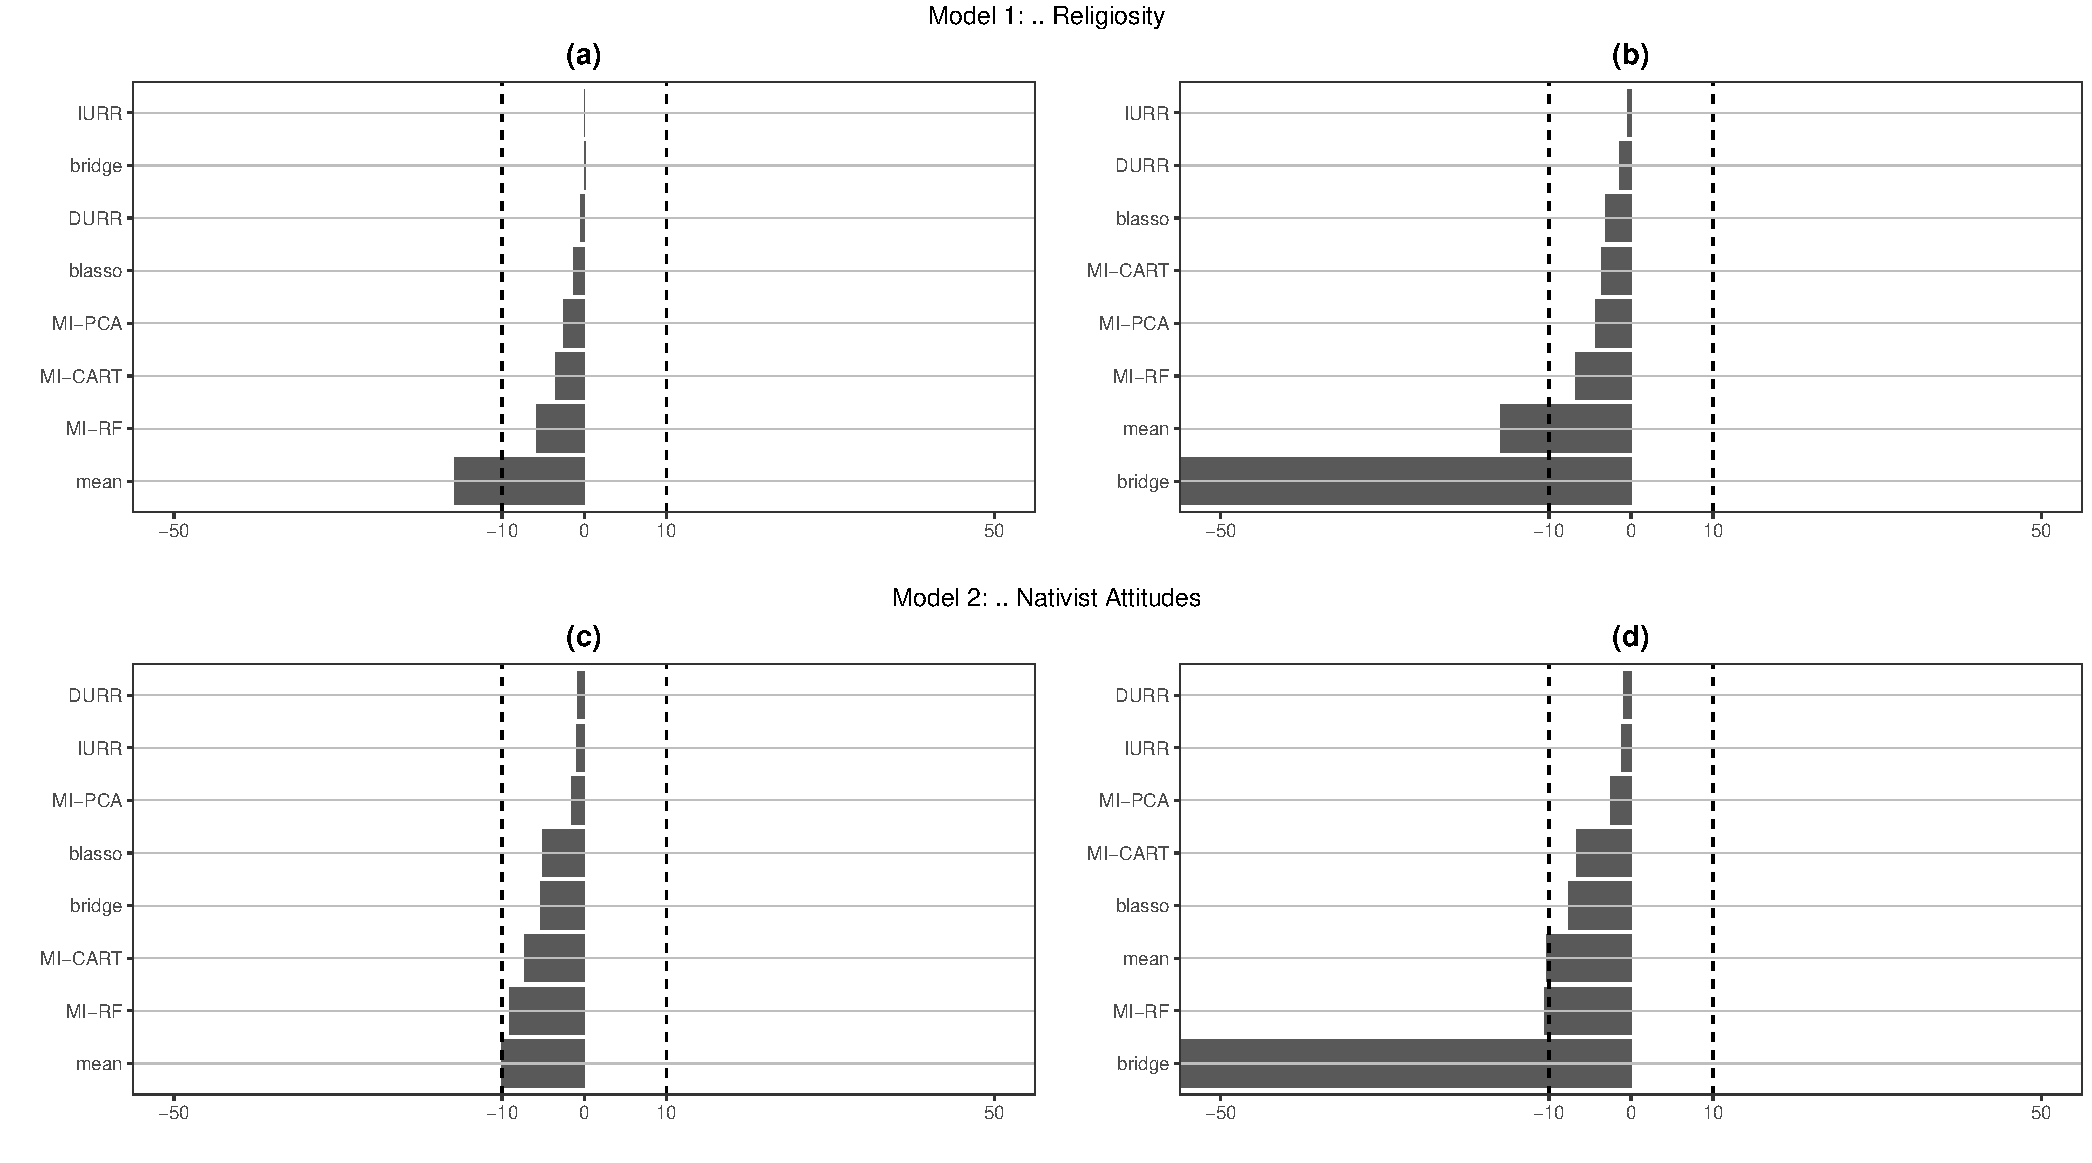
\includegraphics{\pathFIG/exp4_imp_bias.pdf}
	\caption{PRB in the estimation of parameters of interest $\beta^{(1)}_{1}$ and $\beta^{(2)}_{1}$, 
		in model 1 and 2 respectively}
	\label{fig:exp4bias}
\end{figure}

\begin{figure}[h]
	\centering
	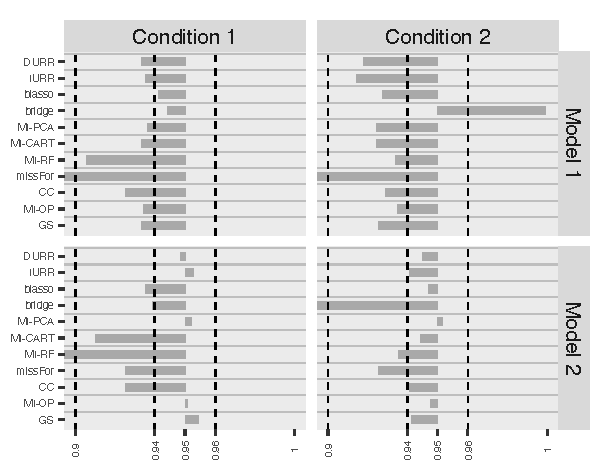
\includegraphics{\pathFIG/exp4_imp_ci.pdf}
	\caption{CIC in the estimation of parameters of interest $\beta^{(1)}_{1}$ and $\beta^{(2)}_{1}$, 
		in model 1 and 2 respectively}
	\label{fig:exp4ci}
\end{figure}

\FloatBarrier

	\subsubsection{Overall Model Parameter Assessment}
	
	Looking at bias and confidence interval coverage for a single parameter of interest can help assess
	the degree to which inferential conclusions, based on it, might change in applied research depending 
	on the imputation method used.
	However, the fitted models were multiple regressions, and the estimate of all model parameters were 
	influenced by the imputations, not only the regression coefficients of some variable of interest.

	Therefore, it is important to observe the overall effects of the different methods on model estimation.
	Figure \ref{fig:exp4_bias_allP} reports the absolute values of the PRBs for each of model 2 parameter 
	estimates, ordered by size, under each of the different missing data treatment considered 
	(see figures \ref{fig:exp4bias_m1} and \ref{fig:exp4cir_m1} in the appendix for model 1 results).
	The figure shows, for each method, how many parameters exceed the 10\% threshold, what is the largest and 
	what is the smallest PRB achieved.

	The regression coefficient for the country dummy code identifying the Netherlands has the largest
	bias across almost all methods and conditions.
	For this reason it is highlighted in the picture, along with the intercept and the focal regression 
	coefficient.

	MI-OP showed that even having perfect information regarding the missing data mechanism and data structure,
	results in some bias for certain estimates.
	Although the bias for the intercept and the focal parameter were negligible, around half of the estimates 
	obtained after using this imputation method showed large biases ($|PRB|>10\%$), and the largest bias was 
	considerable (around 40\%, in the low dimensional condition, and 20\%, in the high-dimensional one).
	
	In both the high- and low-dimensional condition, Multiple Imputation done with DURR, IURR, Blasso, and 
	MI-CART, and single imputation done with missForest showed fairly similar overall patterns to MI-OP, 
	with only slightly larger PRBs.
	MI-PCA and MI-RF also showed similar trends but they presented overall larger PRBs for those estimates 
	exceeding the 10\% threshold.
	However, none of these methods seemed to suffer from the increase in dimensionality.

	Bridge demonstrated the same behaviour described in the simulation studies: it was a competitive method in 
	low dimensional scenarios, but it was inadequate to deal with high-dimensional data imputation (all but 
	one PRBs are larger than 100\%).

	Figure \ref{fig:exp4_ci_allP} reports the confidence interval coverages for each parameter estimate in model 2.
	When using MI-OP, CICs showed a deviation from nominal coverage for only two parameters, with a slight 
	tendency toward over-coverage.
	While DURR, IURR, MI-CART and MI-PCA maintained a similar coverage pattern to the oracle MI-OP approach, 
	blasso, MI-RANF, and missforest were either over- or under-covering many more parameters.
	The behaviour showed by missForest was somewhat to be expected: as a single imputation approach, it 
	underestimates uncertainty regarding values of the empty data cells, and tends to produce narrower
	confidence intervals.

	Despite showing poor performances in terms of bias, Complete Case analysis manifested good 
	coverage.
	However, this was a result of the smaller sample size used for fitting the analysis model, rather than 
	a positive feature of the method: good CI coverage is desirable only as long as bias is contained.

\begin{figure}
	\centering
	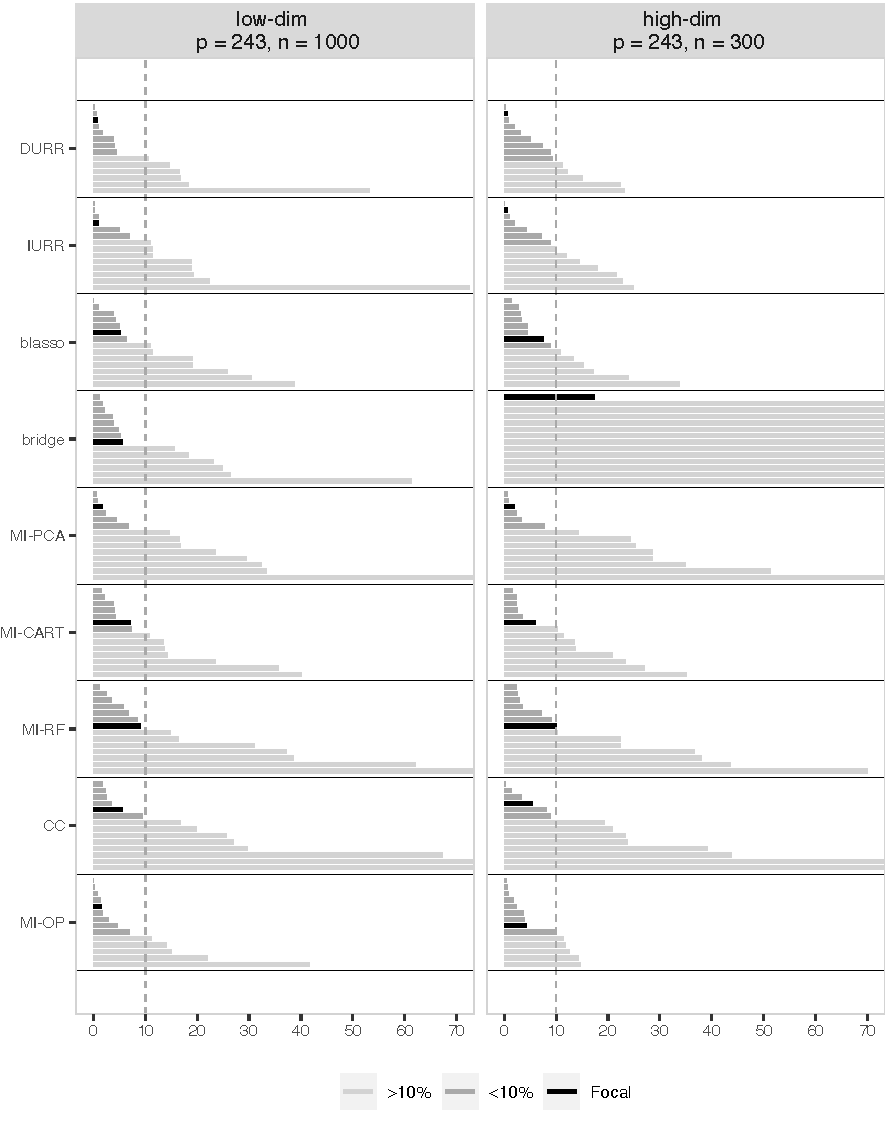
\includegraphics{\pathFIG/exp4_imp_bias_allParms_m2.pdf}
	\caption{PRBs for all the model parameters in model 2. 
		The order of the bars is based on the absolute value of the PRBs.
		The values for the intercept, the focal regression coefficient, and the regression coefficient with which most 
		methods struggle (Largest Bias) are highlighted}
	\label{fig:exp4_bias_allP}
\end{figure}

\begin{figure}
	\centering
	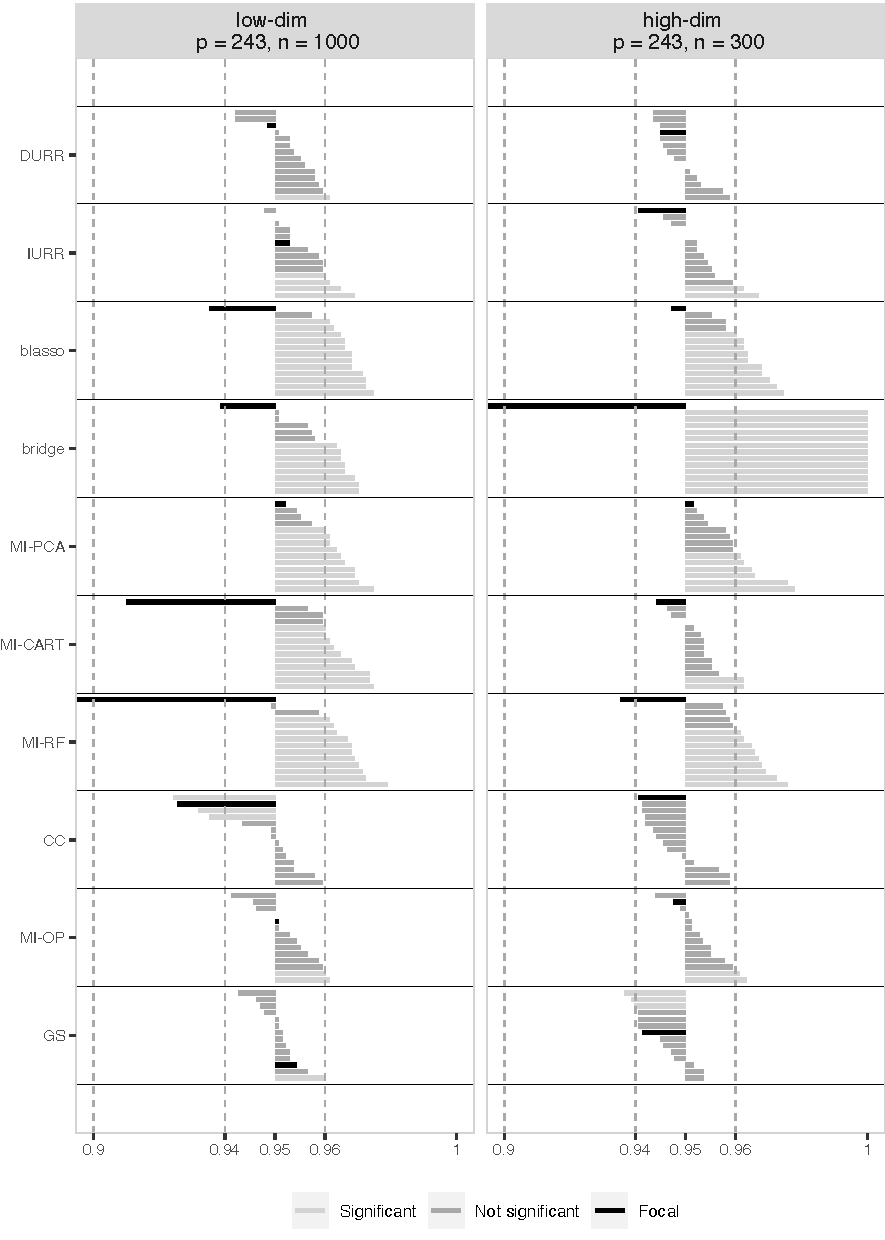
\includegraphics{\pathFIG/exp4_imp_ci_allParms_m2.pdf}
	\caption{CIC for all model parameter in model 2.
		Bars are sorted in by ascending value.
		The values for the intercept, the focal regression coefficient, and the regression coefficient with which most 
		methods struggle (Largest Bias) are highlighted}
	\label{fig:exp4_ci_allP}
\end{figure}

\FloatBarrier

\subsubsection{Imputation Time}

	Table \ref{table:time} reports the average imputation time across the different methods.
	IURR and DURR were the most time consuming methods with imputation times above the hour, 
	in our low dimensional conditions, versus imputation times of a minute or less for MI-PCA and 
	Blasso imputation.
	In the high dimensional condition, IURR and DURR were not as time-intensive, due to the smaller
	sample size, but still required more then ten times the time of MI-PCA and blasso imputation.


\begin{table}[h]
   \begin{center}
\resizebox{\textwidth}{!}{%
        \begin{tabular}{ c c c c c c c c c }
		% Column names
		& \textbf{DURR} & \textbf{IURR} & \textbf{blasso} & \textbf{bridge} & \textbf{MI-PCA} & \textbf{MI-CART} & \textbf{MI-RF} & \textbf{MI-OP} \\ 
		\hline
		% Data
		Condition 1 & 73.20 & 75.90 & 1.40 & 8.10 & 0.60 & 4.00 & 11.30 & 2.20 \\ 
		Condition 2 & 6.10 & 9.70 & 0.50 & 3.20 & 0.40 & 1.40 & 4.70 & 1.90 \\ 
		\hline
        \end{tabular}
}
    \end{center}
\caption{Average imputation time in minutes.} \label{table:time}
\end{table}

\FloatBarrier


